\chapter{\selectlanguage{greek}Μέθοδοι προσομοίωσης}
Στο κεφάλαιο αυτό περιγράφεται η υλοποίηση του συστήματος, με βάση τη μελέτη που παρουσιάστηκε στο προηγούμενο κεφάλαιο. 
Αρχικά παρουσιάζεται η πλατφόρμα και τα προγραμματιστικά εργαλεία που χρησιμοποιήθηκαν. 

\section{Εργαλεία που χρησιμοποιήθηκαν}
Το \en{CST Particle Studio} μπλα μπλα μπλα.

\subsection{Το \en{CST Particle Studio}}
\en{CST PARTICLE STUDIO\textsuperscript{\textregistered} (CST\textsuperscript{\textregistered} PS) is a specialist tool for the fast and accurate analysis of charged particle dynamics in 3D electromagnetic fields.
Powerful and versatile, it is suitable for tasks ranging from designing magnetrons and tuning electron tubes to modeling particle sources and accelerator components.}

\en{The particle tracking solver can model the behavior of particles through static fields, and with the gun iteration, space charge limited emission. 
The particle-in-cell (PIC) solver, which works in the time domain, can perform a fully consistent simulation of particles and electromagnetic fields. 
For relativistic applications, the wakefield solver can calculate how the fields generated by particles traveling at (or close to) the speed of light interact with the structure around them.}

\en{CST PS is integrated with the multi-purpose 3D EM modules of CST STUDIO SUITE\textsuperscript{\textregistered}, such as the CST EM STUDIO\textsuperscript{\textregistered} electro- and magnetostatic solvers and the CST MICROWAVE STUDIO\textsuperscript{\textregistered} eigenmode solver. 
It is fully embedded in the CST STUDIO SUITE design environment, thus benefitting from its intuitive modeling capabilities and powerful import interfaces. 
CST PS is based on the knowledge, research and development that went into the algorithms used in the MAFIA-4 simulation package. 
The powerful PIC solver can also make use of GPU computing, offering significant performance enhancements on compatible hardware.}

\begin{figure}[tph]
\includegraphics[width=0.25\textwidth]{images/CST-logo.png}
\centering
\caption{Το λογότυπο του \en{CST}}
\label{img:CSTlogo}
\end{figure}

\subsection{Το \en{MATLAB}}
Το \en{MATLAB (matrix laboratory)} είναι ένα περιβάλλον αριθμητικής υπολογιστικής και μια προγραμματιστική γλώσσα τέταρτης γενιάς. 
\en{A proprietary programming language developed by MathWorks, MATLAB allows matrix manipulations, plotting of functions and data, implementation of algorithms, creation of user interfaces, and interfacing with programs written in other languages, including C, C++, C\# , Java, Fortran and Python.}

\en{Although MATLAB is intended primarily for numerical computing, an optional toolbox uses the MuPAD symbolic engine, allowing access to symbolic computing abilities. 
An additional package, Simulink, adds graphical multi-domain simulation and model-based design for dynamic and embedded systems.}

\begin{figure}[tph]
\includegraphics[width=0.25\textwidth]{images/Matlab-logo.png}
\centering
\caption{Το λογότυπο του \en{MATLAB}}
\label{img:MATLABlogo}
\end{figure}

\section{Επιρροή διάφορων μεταβλητών σε έναν \en{Electron Beam Scanner}}
Όπως περιγράφεται και από \cite{Logatchov1999}, 

\en{The thin probe beam moves along $X$ axis, is orthogonal to the direction of the relativistic bunch motion ($Z$ axis) with the offset parameter} $\rho$ (Σχήμα \ref{fig:ellipse-EBS}).
\begin{figure}[tph]
\includegraphics{figures/Logatchov1999-EBS}
\centering
\caption{Διαδικασία ανίχνευσης της έλλειψης που χαρακτηρίζει τη δέσμη}
\label{fig:ellipse-EBS}
\end{figure}

\en{The results of scanning are monitored on the screen parallel to the $Y-Z$ plane and positioned at the distance $L$ from $Z$ axis. 
Let the center of the relativistic bunch is located at the origin at time $t=0$ whereas the testing beam has the uniform density along $X$ and the diameter $d \ll \rho$. 
Here, we assume $\rho$ exceeds the typical
transverse size of the relativistic bunch. 
At the time $t=0$ every testing beam particle is corresponded to the certain $x$-coordinate. 
The total deflecting angle in $Y$ direction for every particle under the influence of the electric field of the relativistic bunch can be expressed as:}
		\begin{equation}
			\theta_y (x) = \frac{2 \rho r_e}{\beta} \int_{-\infty}^{\infty}\frac{n(z) \dd z}{\rho^2 + \left(x+\beta z \right) ^2}
		\end{equation}
\en{where $r_e$ is the classical electron radius, $\beta =v_t/c$ - the relative velocity of the testing beam, $c$ - the velocity of light, $x$ - the coordinate of testing beam particle at $t=0$, $n(z)$ - the relativistic bunch linear density along $Z$ axis. 
The expression for the deflecting angle of the particle in $Z$ direction due to magnetic field can be written as:}
		
		\begin{equation}
			\theta_z(x) = 2 r_e \int_{-\infty}^{\infty}\frac{(x+\beta z)n(z) \dd z}{\rho^2 + \left(x+\beta z \right) ^2}
		\end{equation}
		Αυτά τα κάνουμε \en{plot} και είδαμε πώς επηρεάζονται από 
		\begin{itemize}
			\item \en{bunch intensity}
			\item \en{bunch length}
			\item \en{Y-offset} ($\rho$) 
			\item \en{probe beam voltage} 
		\end{itemize}   

\begin{figure}[tbh]
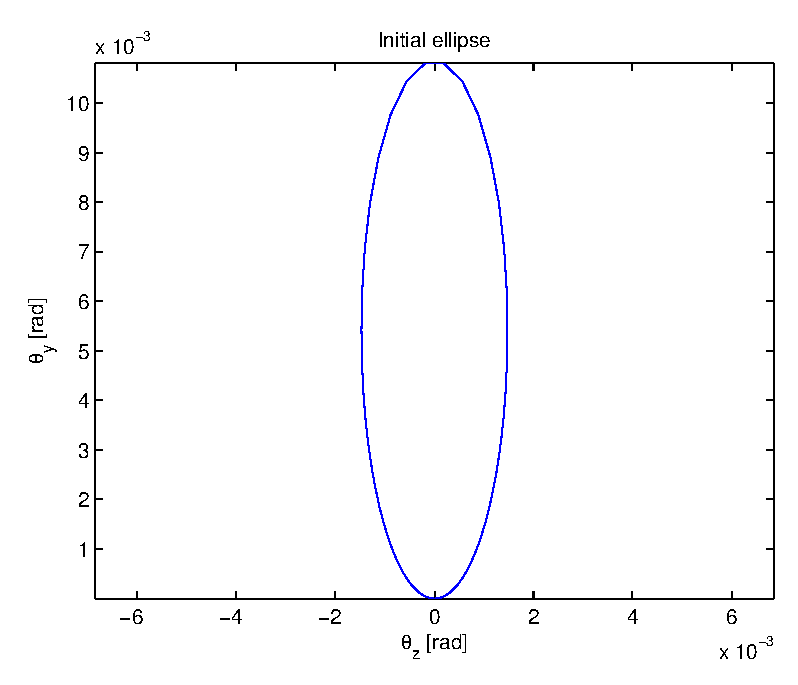
\includegraphics[width=0.75\textwidth]{figures/beam_deflection_script_01_initial_elipse}
\centering
\caption{Έλλειψη στην αρχική κατάσταση}
\label{fig:beam_deflection_script_01_initial_elipse}
\end{figure}

\begin{figure}[tbh]
\includegraphics[width=0.75\textwidth]{figures/beam_deflection_script_02_elipse_width}
\centering
\caption{Το πλάτος και ύψος της έλλειψης στην αρχική κατάσταση}
\label{fig:beam_deflection_script_02_elipse_width}
\end{figure}

\begin{figure}[tbh]
\includegraphics[width=0.75\textwidth]{figures/beam_deflection_script_03_elipse_height}
\centering
\caption{Επιρροή της έντασης της δέσμης στην ύψος και το λόγο της έλλειψης}
\label{fig:beam_deflection_script_03_elipse_height}
\end{figure}

\begin{figure}[tbh]
\includegraphics[width=0.75\textwidth]{figures/beam_deflection_script_04_elipse_height_by_bunch_intensity}
\centering
\caption{Επιρροή του μήκους της δέσμης στην ύψος και το λόγο της έλλειψης}
\label{fig:beam_deflection_script_04_elipse_height_by_bunch_intensity}
\end{figure}

\begin{figure}[tbh]
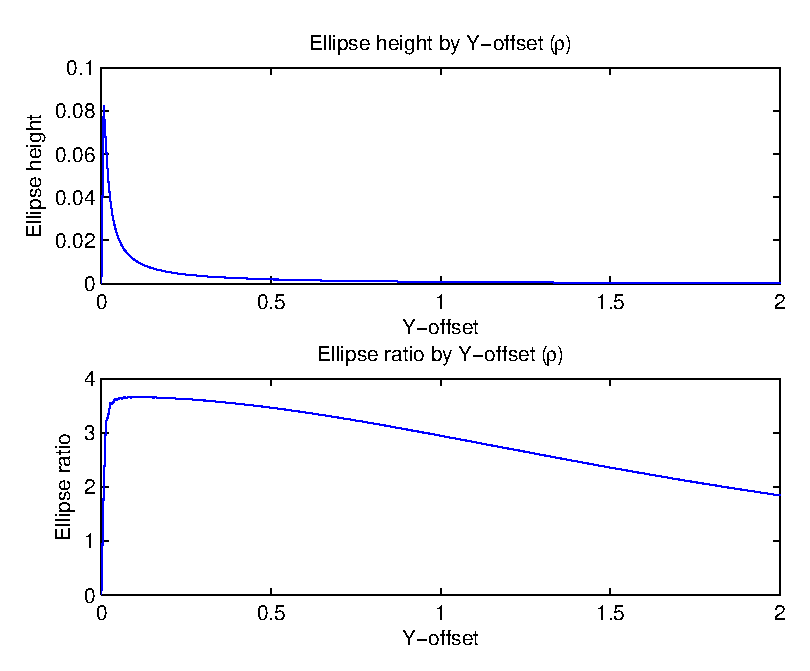
\includegraphics[width=0.75\textwidth]{figures/beam_deflection_script_05_elipse_ratio_by_bunch_intensity}
\centering
\caption{Επιρροή της αρχικής θέσης ριπής ($Y$-\en{offset} της δέσμης στην ύψος και το λόγο της έλλειψης}
\label{fig:beam_deflection_script_05_elipse_ratio_by_bunch_intensity}
\end{figure}

\begin{figure}[tbh]
\includegraphics[width=0.75\textwidth]{figures/beam_deflection_script_06}
\centering
\caption{Επιρροή της γραμμικής μεταβολής τάσης της δέσμης στην ύψος και το λόγο της έλλειψης}
\label{fig:beam_deflection_script_06}
\end{figure}

\begin{figure}[tbh]
\includegraphics[width=0.75\textwidth]{figures/beam_deflection_script_07}
\centering
\caption{Επιρροή της εκθετικής μεταβολής τάσης της δέσμης στην ύψος και το λόγο της έλλειψης}
\label{fig:beam_deflection_script_07}
\end{figure}

\section{Ανάλυση με το \en{CST Particle Studio}}

\begin{figure}[tbh]
\includegraphics[width=0.5\textwidth]{figures/CST-main-beam-source}
\centering
\caption{Η πηγή της δέσμης στο \en{CST}}
\label{fig:CST-mainBeamSource}
\end{figure}

\begin{figure}[tbh]
\includegraphics[width=\textwidth]{figures/CST-pic-monitor}
\centering
\caption{Η διάταξη προσομοιωμένη στο \en{CST}}
\label{fig:CST-PICmonitor}
\end{figure}
